\documentclass[13pt,oneside]{book}
\usepackage[utf8]{inputenc}
\usepackage{url}
\usepackage{listings}
\usepackage{graphicx}

\usepackage{geometry}
\geometry{a4paper, left=20mm, right=20mm, top=20mm, bottom=20mm}
\usepackage[toc,page]{appendix}
\usepackage{graphicx}
\usepackage{natbib}
\usepackage{lipsum}
\usepackage{caption}

\begin{document}

\captionsetup[figure]{margin=1.5cm,font=small,labelfont={bf},name={Figure},labelsep=colon,textfont={it}}
\captionsetup[table]{margin=1.5cm,font=small,labelfont={bf},name={Table},labelsep=colon,textfont={it}}
\setlipsumdefault{1}

\begin{titlepage}
\begin{center}
{\LARGE College Of Engineering Trivandrum}\\[3cm]
\linespread{1.2}\huge {\bfseries System Software Lab}\\[3cm]
\linespread{1}

\includegraphics[width=5cm]{img/emblem.jpeg}\\[3cm]
{\Large GOKUL K\\ S5  CSE \\ Roll No:21\\ TVE18CS021 }\\[1cm]


\textit{ }\\[2cm]
Department of Computer Science\\[0.2cm]
\today
\end{center}

\end{titlepage}

\newpage

\begin{frame}{}
    \centering
    \hspace*{-0.5cm}
    $\vcenter{\hbox{
\includegraphics[width=1.5cm]{img/emblem.jpeg}}}$
    $\vcenter{\resizebox{0.95\textwidth}{!}{
        \begin{tabular}{c}
             CS331 - System Software Lab $\cdot$ 2020 $\cdot$   \\
             \hline 
        \end{tabular}
    }}$
\end{frame}
\section*{Cycle 1}
\section*{Expt 7}
\begin{center}
    \Large{File Organisation Techniques}
\end{center}
\section*{Aim}
\large
Simulate the following file organization techniques:\\
 a) Single level directory\\
 b) Two level directory\\
 c) Hierarchical\\
\section*{Algorithm} 
\subsection{Single Level}
In a single-level directory system, all the files are placed in one directory. There
is a root directory which has all files. It has a simple architecture and there are no
sub directories. Advantage of single-level directory system is that it is easy to find
a file in the directory. A single-level directory has significant limitations, however,
when the number of files increases or when the system has more than one user. Since
all files are in the same directory, they must have unique names.
\subsection{Two Level}
In the two-level directory system, each user has own user file directory (UFD).
The system maintains a master block that has one entry for each user. This master
block contains the addresses of the directory of the users. When a user job starts
or a user logs in, the system’s master file directory (MFD) is searched. When a
user refers to a particular file, only his own UFD is searched. This effectively solves
the name collision problem and isolates users from one another. Isolation is an ad-
vantage when the users are completely independent but is a disadvantage when the
users want to cooperate on some task and to access one another’s files.
\subsection{Hierarchical}
Hierarchical directory structure, also called a tree-structured directory allows
users to create their own subdirectories and to organize their files accordingly. A
tree is the most common directory structure. The tree has a root directory, and
every file in the system has a unique path name. A directory (or subdirectory)
contains a set of files or subdirectories.


\section*{Source Code}
\small
\subsection{FSObject.h}
\begin{lstlisting}[language=C]
#ifndef _FSOBJECT
#define _FSOBJECT

#define MAX_CHILDREN 25
#define PWD_STACK_LENGTH 100

typedef enum { DIR, FIL } FSObjectType;

typedef enum { SINGLE, DOUBLE, HIERARCHIAL } FilesystemType;

struct FileSystemObject {
  char name[255];
  FSObjectType type;
  struct FileSystemObject *children[MAX_CHILDREN];
  int no_of_children;
};

typedef struct FileSystemObject FSObject;

typedef struct {
  FSObject *root;
  FSObject *wd[PWD_STACK_LENGTH];
  int pwd_depth;
  FilesystemType fs_type;
} Filesystem;

void pwd(Filesystem *);
void mkdir(Filesystem *, char[255]);
void cd(Filesystem *, char[255]);
void touch(Filesystem *, char[255]);
void ls(Filesystem *);

#endif
    \end{lstlisting}
\subsection{FSObject.c}
\begin{lstlisting}[language=C]
#include "FSObject.h"
#include <stdio.h>
#include <stdlib.h>
#include <string.h>

// Prints the location of present directory
void pwd(Filesystem *fs) {
  printf("/");
  for (int i = 0; i < (fs->pwd_depth) + 1; i++) {
    printf("%s/", fs->wd[i]->name);
  }
}

// Creates a new directory in pwd
void mkdir(Filesystem *fs, char name[255]) {
  FSObject *pwd = fs->wd[fs->pwd_depth];

  if (pwd->no_of_children == MAX_CHILDREN || fs->fs_type == SINGLE ||
      (fs->fs_type == DOUBLE && fs->pwd_depth == 1)) {
    printf("Cannot create a new directory\n");
    return;
  } else {
    FSObject *new_dir = malloc(sizeof(FSObject));
    new_dir->type = DIR;
    strcpy(new_dir->name, name);
    new_dir->no_of_children = 0;

    pwd->children[pwd->no_of_children] = new_dir;
    pwd->no_of_children += 1;
  }
}

// Change directory to a child of pwd
void cd(Filesystem *fs, char name[255]) {
  FSObject *pwd = fs->wd[fs->pwd_depth];

  if (strcmp(name, "..") == 0) {
    fs->pwd_depth -= 1;
  } else if (fs->pwd_depth == PWD_STACK_LENGTH) {
    printf("Cannot cd. Maximum stack length reached\n");
    return;
  } else {
    for (int i = 0; i < pwd->no_of_children; i++) {
      if (strcmp(pwd->children[i]->name, name) == 0 &&
          pwd->children[i]->type == DIR) {
        fs->pwd_depth += 1;
        fs->wd[fs->pwd_depth] = pwd->children[i];
        return;
      }
    }
    printf("No directory named %s in %s\n", name, pwd->name);
  }
}

// Create a new file in pwd
void touch(Filesystem *fs, char name[255]) {
  FSObject *pwd = fs->wd[fs->pwd_depth];

  if (pwd->no_of_children == MAX_CHILDREN) {
    printf("Cannot create file. Max children reached\n");
    return;
  }

  FSObject *new_file = malloc(sizeof(FSObject));
  new_file->type = FIL;
  strcpy(new_file->name, name);

  pwd->children[pwd->no_of_children] = new_file;
  pwd->no_of_children += 1;
}

// List all files and folders in pwd
void ls(Filesystem *fs) {
  FSObject *pwd = fs->wd[fs->pwd_depth];

  for (int i = 0; i < pwd->no_of_children; i++)
    if (pwd->children[i]->type == DIR)
      printf("%s/\t", pwd->children[i]->name);
    else
      printf("%s\t", pwd->children[i]->name);

  printf("\n");
  return;
}
    \end{lstlisting}
\subsection{main.c}
\begin{lstlisting}[language=C]
#include "FSObject.h"
#include <stdio.h>
#include <stdlib.h>
#include <string.h>

FSObject *init_root_dir(char name[255]) {
  FSObject *root_folder = malloc(sizeof(FSObject));
  strcpy(root_folder->name, name);
  root_folder->type = DIR;
  root_folder->no_of_children = 0;

  return root_folder;
}

Filesystem *init_fs(FilesystemType fs_type, FSObject *root_folder) {
  Filesystem *filesystem = malloc(sizeof(filesystem));
  filesystem->root = root_folder;
  filesystem->fs_type = fs_type;
  filesystem->wd[0] = root_folder;
  filesystem->pwd_depth = 0;

  return filesystem;
}

int main() {
  int choice;
  char command[5], operand[255];
  Filesystem *filesystem;
  FSObject *root_dir;
  FilesystemType fs_type;

  printf("Enter type of filesystem\n1. Single\t 2. Double\t 3. Hierarchial\n");
  scanf("%d", &choice);

  switch (choice) {
  case 1:
    fs_type = SINGLE;
    break;

  case 2:
    fs_type = DOUBLE;
    break;

  case 3:
    fs_type = HIERARCHIAL;
    break;

  default:
    printf("Unknown type\n");
    exit(0);
  }

  printf("Enter root directory name: ");
  scanf("%s", operand);

  root_dir = init_root_dir(operand);
  filesystem = init_fs(fs_type, root_dir);

  printf("\n\nList of available commands:\n"
         "pwd\tls\tmkdir\ttouch\tcd\texit\n");

  while (strcmp(command, "exit") != 0) {

    pwd(filesystem);
    printf(">> ");
    scanf("%s", command);

    if (strcmp(command, "pwd") == 0) {
      pwd(filesystem);
      printf("\n");
    } else if (strcmp(command, "ls") == 0)
      ls(filesystem);
    else if (strcmp(command, "touch") == 0) {
      scanf("%s", operand);
      touch(filesystem, operand);
    } else if (strcmp(command, "mkdir") == 0) {
      scanf("%s", operand);
      mkdir(filesystem, operand);
    } else if (strcmp(command, "cd") == 0) {
      scanf("%s", operand);
      cd(filesystem, operand);
    }  else if (strcmp(command, "exit") == 0) {
		continue;
    } else {
      printf("Unknown command %s\n", command);
    }
  	printf("\n");
  }

  return 0;
}
    \end{lstlisting}
    \section*{Output}
    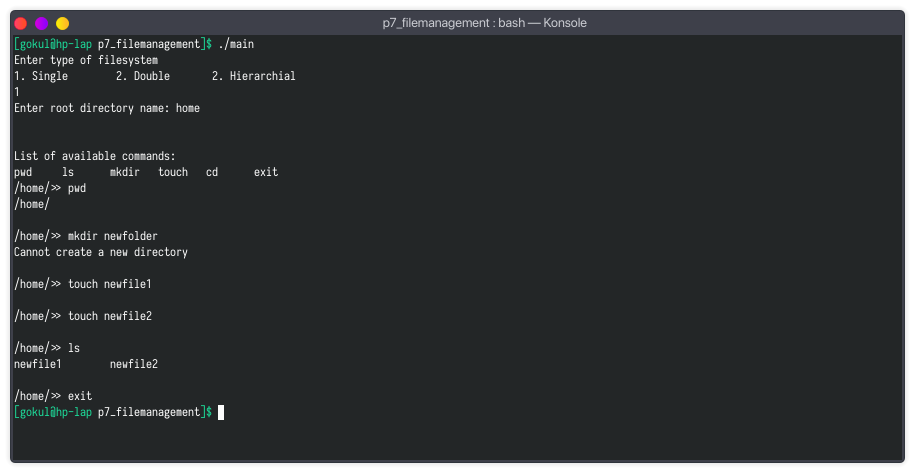
\includegraphics[width=\textwidth]{img/p7/ss1.png}
    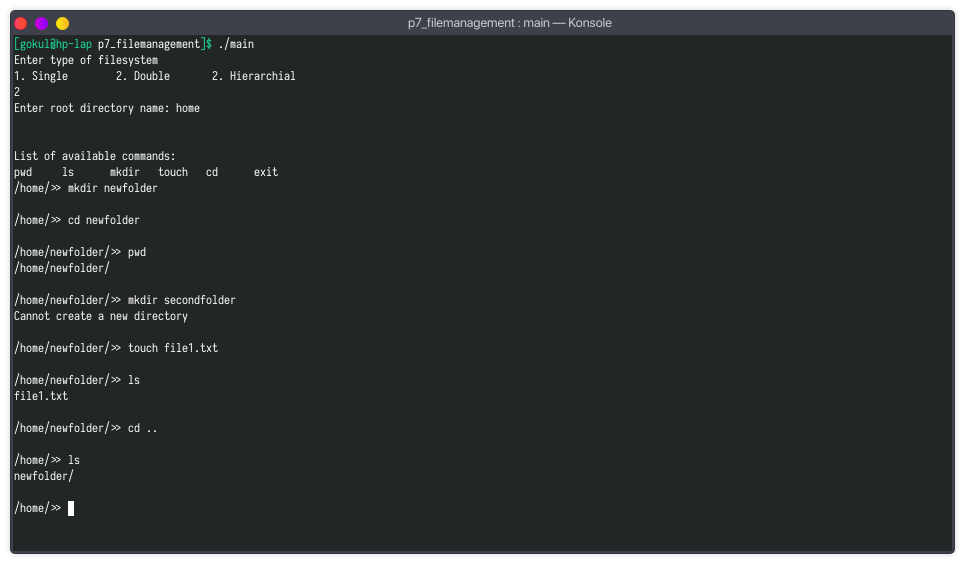
\includegraphics[width=\textwidth]{img/p7/ss2.png}
    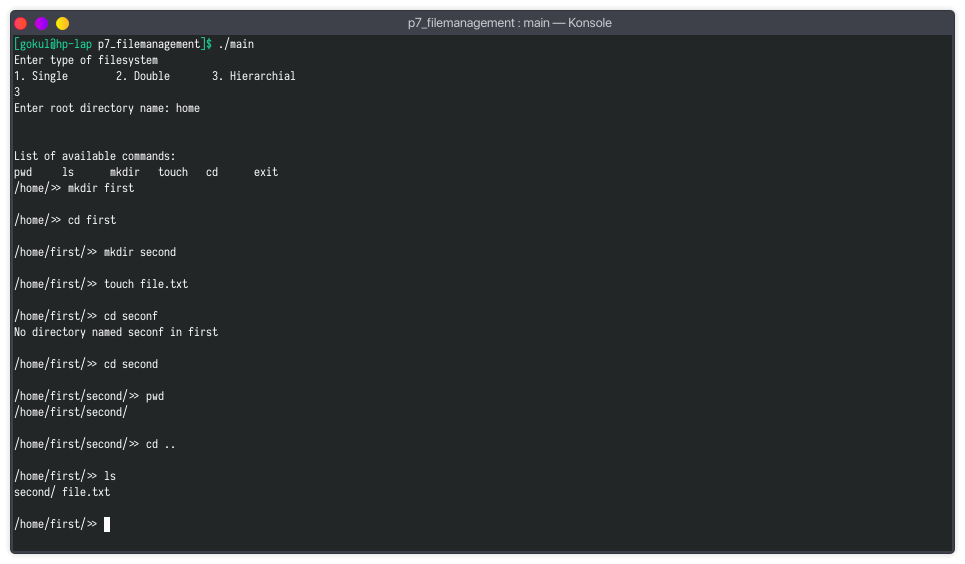
\includegraphics[width=\textwidth]{img/p7/ss3.png}
\Large
\section*{Result}
\large
Basic file organisation techniques was simulated and its output verified
\end{document}